\documentclass[eng]{csam}
\usepackage{graphicx}
\usepackage{natbib}
\usepackage{amsmath,multirow}
\usepackage{enumerate,array}
\usepackage{xcolor}
\usepackage[ruled,vlined]{algorithm2e}

\def \bY { \mathbf{ Y } }
\def \bX { \mathbf{ X } }
\def \bU { \mathbf{ U } }
\def \bmu { \boldsymbol{ \mu } }
\def \bSigma { \boldsymbol{ \Sigma } } 
\def \bphi { \boldsymbol{ \phi } }
\def \bepsilon { \boldsymbol{ \epsilon } }

%% ==================================================================
%% Templete File for Communications of the Korean Statistical Society
%% Korean Statistical Society (office@kss.or.kr)
%% ==================================================================

%%\submit{draft}
% ==================== Do not Modify here ============================
\submit{final}
\volumn{20}{1}{2013}
\receive{0000}{00}{00} \revise{0000}{00}{00}  \accept{0000}{00}{00}
\setpagenum{1}
% ====================================================================


\heading{Bootstrap aggregated classification for sparse functional data}{Hyunsung Kim, Yaeji Lim}

\begin{document}

\title{Bootstrap aggregated classification for sparse functional data}

\author{Hyunsung Kim\address[a]{Department of Statistics, Chung-Ang University, Korea}, 
	Yaeji Lim\footnote{Corresponding author: Professor, Department of Applied Statistics, Chung-Ang University, 84 Heukseok-ro, Dongjak-gu, Seoul 06974, Korea. E-mail: yaeji.lim@gmail.com}\address[b]{Department of Applied Statistics, Chung-Ang University, Korea}}

\begin{abstract}
	{\color{red}
		Abstract
	}
\end{abstract}

\keywords{functional principal component analysis, bootstrap aggregating, classification}

\section{Introduction}
{\color{red} 
	Prior studies
	
	Description of sections
}


\section{Preliminaries}
\subsection{Functional principal compnent analysis}
Functional data analysis (FDA) is a kind of statistics that analyzes the curves or functions rather than single points.
In FDA, data (or curve) is defined on the infinite dimension, so dimensionality reduction becomes a key issue. One of the popular dimension reduction method in FDA is functional principal component analysis (FPCA) which finds directions of the variation and exploits by data-driven basis called functional principal component (FPC) scores. 

%Let $X(t)$ is a square integrable random process for $t \in \mathcal{T}$ with mean function $\mu(t) = E\big(X(t)\big)$ and covariance function $G(s,t) = \text{cov}\big(X(s),X(t)\big)$ for $s, t \in \mathcal{T}$.
Let $X(t)$, defined on finite $\mathcal{T}$, is a square integrable random process which means $X(\cdot) \in L_2(\mathcal{T})$ with mean function $\mu(t) = E\big(X(t)\big)$ and covariance function $G(s,t) = \text{cov}\big(X(s),X(t)\big)$ for $s, t \in \mathcal{T}$.
By Mercer's theorem, the covariance function can be represented by $G(s,t) = \sum_{k=1}^\infty \lambda_k \phi_k(s) \phi_k(t)$ where $\lambda_1 \ge \lambda_2 \ge \dots \ge 0 $ are non-negative eigenvalues satisfying $\sum_{k=1}^\infty \lambda_k < \infty$ and $\phi_k$'s are the corresponding orthonormal eigenfunctions.
By the Karhunen-Lo\`{e}ve expansion, the $i$th random curve can be represented as
\begin{equation}
X_i(t) = \mu(t) + \sum_{k=1}^\infty \xi_{ik} \phi_k(t), \hspace{0.5cm} t \in \mathcal{T}
\end{equation}
where $\xi_{ik} = \int_{\mathcal{T}} \big( X_i(t) - \mu(t) \big)\phi_k(t) dt $ are uncorrelated variables with mean 0 and variance $\lambda_k$.
%$E(\xi_{ik}) = 0$, $E(\xi_{ij} \xi_{ik}) = 0$ for $j \ne k$, and $E(\xi_{ik}^2) = \lambda_k$.

In the real world, functional data is observed with measurement errors. Then the $i$th curve with random noise is 
\begin{align}
U_i(t) &= X_i(t) + \epsilon_i(t) \nonumber \\
&= \mu(t) + \sum_{k=1}^\infty \xi_{ik} \phi_k(t) + \epsilon_i(t), \hspace{0.5cm} t \in \mathcal{T}
\end{align}
where $\epsilon_i(t)$ are the uncorrelated measurement errors with mean 0 and variance $\sigma^2$.

{\color{red}
	PC selection? PVE, AIC, BIC, truncation number(size) $K$
}


\subsection{Functional principal component analysis for sparse functional data}
Let $t_{ij} \in \mathcal{T}$ is the $j$th time point observed in the $i$th curve $X_i$ where $i = 1, 2, \dots, n$, $j = 1, 2, \dots, n_i$.
Then, the $i$th curve for sparse functional data can be expressed as
\begin{equation}
%\bY_i = \bmu_i + \sum_{k=1}^\infty \xi_{ik} \bphi_{ik} + \bepsilon_i.
U_i(t_{ij}) = \mu(t_{ij}) + \sum_{k=1}^\infty \xi_{ik} \phi_k(t_{ij}) + \epsilon_i(t_{ij}), \hspace{0.5cm} t_{ij} \in \mathcal{T}
\end{equation}
where $\epsilon_i(t_{ij})$ are the random noises.
%Then the $i$th curve for sparse functional data is
%\begin{align}
%	Y_i(t_{ij}) &= X_i(t_{ij}) + \epsilon_i(t_{ij}) \nonumber \\
%			    &= \mu(t_{ij}) + \sum_{k=1}^\infty \xi_{ik} \phi_k(t_{ij}) + \epsilon_i(t_{ij}), \hspace{0.5cm} t_{ij} \in \mathcal{T}
%\end{align}

In dense functional data which means that data is observed at regular grid, we can estimate the FPC scores by numerical integration directly. 
On the other hand, when each curve is observed at sparse or irregular time points, estimating the FPC scores by numerical integration is not appropriate since the estimate of $\xi_{ik}$ would be biased. To overcome this problem, Yao {\em et al.} (2005) proposed principal component analysis through conditional expectation (PACE) method.
Let $\bX_i = \big( X_i(t_{i1}), \dots, X_i(t_{in_i}) \big)^T$, $\bU_i = \big( U_i(t_{in_1}), \dots, U_i(t_{in_i}) \big)^T$, $\bmu_i = \big( \mu(t_{i1}), \dots, \mu(t_{in_i}) \big)^T$, $\bphi_{ik} = \big( \phi_k(t_{i1}), \dots, \phi_k(t_{in_i}) \big)^T$, and $\bepsilon_i = \big( \epsilon_i(t_{i1}), \dots, \epsilon_i(t_{in_i}) \big)^T$.
The best linear unbiased prediction (BLUP) of $\xi_{ik}$, $k$th FPC scores of $i$th subject, by PACE is
\begin{equation}
\tilde \xi_{ik} = E[\xi_{ik} \vert \bU_i] = \lambda_k \bphi_{ik}^T\bSigma_{\bU_i}^{-1}(\bU_i - \bmu_i),
\end{equation}
where $\bSigma_{\bU_i} = \text{cov}(\bU_i, \bU_i) = \text{cov}(\bX_i, \bX_i) + \sigma^2\mathbf{I}_{n_i}$,

From the above, the PACE estimate of $\xi_{ik}$ is obtained as follow
\begin{equation}
\hat \xi_{ik} = \widehat E[\xi_{ik} \vert \bU_i] = \hat\lambda_k \hat\bphi_{ik}^T \widehat\bSigma_{\bU_i}^{-1}(\bU_i - \hat\bmu_i).
\end{equation}
where $\widehat\bSigma_{\bU_i} = \widehat{\text{cov}}(\bU_i, \bU_i) = \widehat{\text{cov}}(\bX_i, \bX_i) + \hat\sigma^2\mathbf{I}_{n_i}$


{\color{red}
	How to apply FPCA for sparse data?
}



\section{Method}
\subsection{Functional classification(Classification based on functional principal component scores)}
Let $X_i(\cdot)$ is the $i$th curve, $Y_i$ is its class response, $\beta(\cdot)$ is the weight function and $\epsilon_i$ is the $i$th random error.
Then, the functional linear model (FLM) is
\begin{equation}
Y_i = \int_{\mathcal{T}} X_i(t) \beta(t) dt + \epsilon_i.
\end{equation}
If we use the FPCA form that means $X_i(t) = \sum_{k=1}^\infty \xi_{ik} \phi_k(t_{ij})$ and $\beta(t) = \sum_{k=1}^\infty \beta_k \phi_k(t_{ij})$, then the FLM is represented by
\begin{align}
Y_i &= \sum_{k=1}^\infty \beta_k \xi_{ik} + \epsilon_i \nonumber \\
&\approx \sum_{k=1}^K \beta_k \xi_{ik} + \epsilon_i,
\end{align}
where $K$ is the truncated number on FPCA.

\subsection{Bootstrap aggregating}
Bootstrap aggregating (Bagging) is the ensemble method using bootstrap ideas proposed by Breiman (1996).
It is known to improve performance of the classifier and reduce the variance by aggregating predictions from each bootstrap resample.
Suppose there are $K$ response classes with $C_1, \dots, C_K$ and $\hat f^{(b)}(x)$ for $b=1, \dots, B$ be a classifier obtained by $b$th bootstrap resample.
Then, the estimate of bagged classifier using the majority vote scheme is
\begin{equation}
\hat y_{\text{bag}} = \arg\max_j \# \big\{ b \lvert \hat f^{(b)}(x) = C_j \big\}.
\end{equation}

{\color{red}
	What is bagging?
}


\subsection{Bootstrap aggregated classifier with sparse FPCA}
The proposed method is bootstrap aggregated classification with FPCA for sparse functional data. 
Suppose we have $n$ curves with $K$ different class label denoted by $\mathcal{D} = \big\{(\bU_1, y_1), \dots, (\bU_n, y_n) \big\}$.
Denote $\mathcal{D}^{(b)} = \big\{(\bU^{(b)}_1, y^{(b)}_1), \dots, (\bU^{(b)}_n, y^{(b)}_n) \big\}$ is a $b$th bootstrap resample.

The summary of procedure is below algorithm.

\begin{algorithm}[H]
	\caption{Bagged classifier with sparse FPCA}
	\begin{enumerate}
		\item For $b = 1, \dots, B$, repeat
		\begin{enumerate}
			\item Generate a bootstrap resample $\mathcal{D}^{(b)}$ from the data $\mathcal{D}$.
			\item Apply functional principal component analysis for $\mathcal{D}^{(b)}$.
			\item Estimate the FPC scores by PACE.
			\item Select $K$, the number of FPCs, such that PVE $\ge 0.99$.
			\item Construct classifier on $K$ FPC scores.
		\end{enumerate}
%		\item Given a new curve $\bU^*$, obtain each $B$ predictions from above $B$ classifiers.
		\item Given a new curve $\bU^*$, for $b = 1, \dots, B$, repeat
		\begin{enumerate}
			\item Estimate the FPC scores by PACE using FPC function from $\mathcal{D}_{b}$.
			\item Obtain the prediction $\hat y^{(b)}$ from above $b$th classifiers.
		\end{enumerate}
	
		\item From $\hat y^{(1)}, \dots, \hat y^{(B)}$, obtain the final prediction $\hat y_{bag}$ aggreated by majority vote.
	\end{enumerate}
\end{algorithm}

{\color{red}
	algorithm flow
	
	algorithm image
	
	What is the proposed method?
}




\section{Simulation studies}
{\color{red}
	Data generating
	
	Result
}


%\begin{table}[t]
%\footnotesize
%\centering
%\caption{Structure of data.}\label{tb:data1}
%\tabcolsep=35.5pt
%\begin{tabular}{ccccc}
%\hline \hline
%\multirow{2}*{$N$} & \multicolumn{4}{c}{factor level} \\\cline{2-5}
% & 1 & 2 & $\cdots$ & $I$ \\\hline
%1        & $x_{11}$ & $x_{21}$ & $\cdots$ & $x_{I1}$ \\
%2        & $x_{12}$ & $x_{22}$ & $\cdots$ & $x_{I2}$ \\
%$\vdots$ & $\vdots$ & $\vdots$ & $\ddots$ & $\vdots$ \\
%$n$      & $x_{1n}$ & $x_{2n}$ & $\cdots$ & $x_{In}$ \\
%\hline \hline
%\end{tabular}
%\end{table}


\section{Real data analysis}
\subsection{Berkely growth data}
We apply the proposed method to the berkely growth data presented in Tuddenham \& Snyder (1954). 
The dataset was measured height for 93 individuals, 54 girls and 39 boys. There are 31 observations from ages 1 to 18 for each curve.
These dense curves with 54 girls and 39 boys are plotted in Figure 1.

\begin{figure}[h]
	\centering
	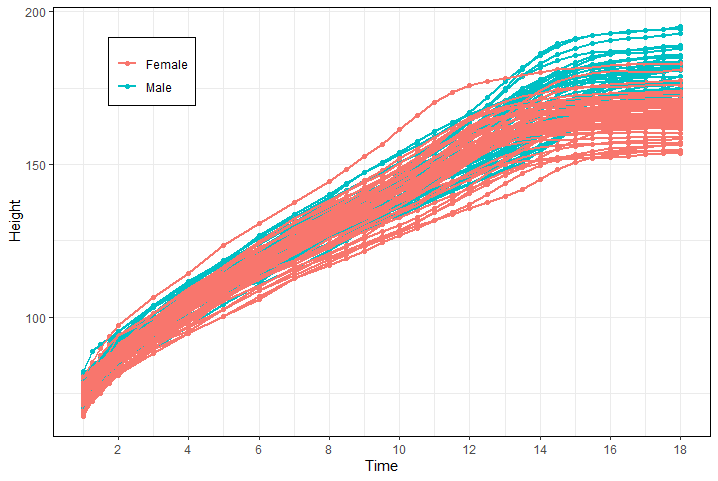
\includegraphics[height=4cm,keepaspectratio=true]{img/growth.png}
	\caption{The berkely growth data of 93 individuals.}
	\label{fig:rsxb}
\end{figure}

\begin{table}[ht]
	\footnotesize
	\centering
	\caption{The average classification error with standard error in percentage from 100 Monte Carlo repetitions for berkerly growth data}
	\tabcolsep=11.5pt
	\begin{tabular}{ccccccc}
		\hline \hline
		& Logistic   & SVM      & SVM        &     &     & Naive \\
		Method & Regression & (Linear) & (Gaussian) & LDA & QDA & Bayes \\ 
		\hline
		Single        & 7.3 (4.80) & 5.3 (3.20) & 5.7 (4.03) & 5.8 (3.34) & 5.6 (3.35) & 5.6 (3.90) \\ 
		Majority vote & 5.9 (4.12) & 4.9 (3.19) & 5.3 (3.51) & 5.4 (3.24) & 4.9 (3.57) & 5.5 (3.96) \\ 
		OOB weight    & 5.9 (4.12) & 5.0 (3.22) & 5.4 (3.62) & 5.4 (3.27) & 4.9 (3.54) & 5.5 (3.96) \\ 
		\hline \hline
	\end{tabular}
\end{table}

{\color{red}
	Data description
	
	Result	
}


\subsection{Spinal bone mineral density data}
We apply the proposed method to the spinal bone mineral density data presented in Bachrach {\em et al.} (1999). The dataset has the spinal bone mineral density for 280 individuals, 153 females and 127 males measured at sparse and irregualar time points. There are 2~4 observations for each curve. The dataset has also ethnicity information such that Asian, Black, Hispanic and White. These sparse curves with 153 females and 127 males are plotted in Figure 2.
\begin{figure}[h]
	\centering
	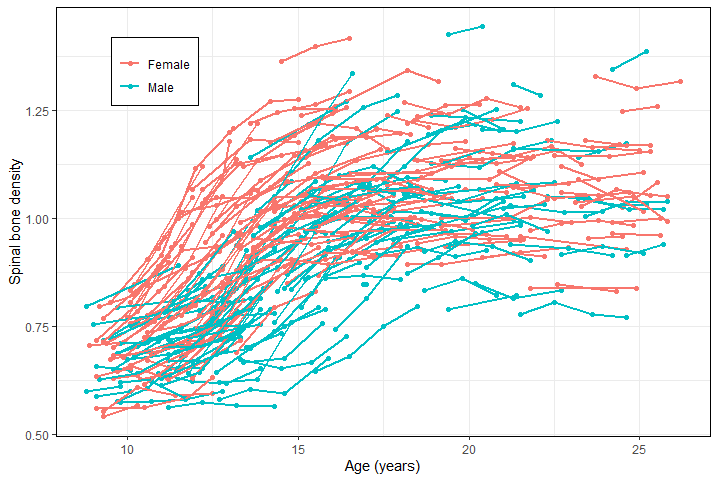
\includegraphics[height=4cm,keepaspectratio=true]{img/spnbmd.png}
	\caption{The spinal bone mineral density of 280 individuals.}
	\label{fig:rsxb}
\end{figure}

We try to classify gender for proposed method. First, we split the sparse spinal bone mineral density data to training and test set. We generate 100 bootstrap resamples from training set. We applied FPCA with PACE for each bootstrap resample to obtain the FPC scores. We construct 100 classifiers on FPC scores from each bootstrap resample. From test set, 100 bootstrap predictions are obtained for each curve. Then we get the final prediction by majority vote from 100 bootstrap predictions. We repeat 100 times with different seeds for different split of training and test set. 
%James \& Hastie (2001) proposed functional linear discriminant analysis (FLDA) to 

\begin{table}[ht]
	\footnotesize
	\centering
	\caption{The average classification error with standard error in percentage from 100 Monte Carlo repetitions for spinal bone mineral density data}
	\tabcolsep=10.5pt
	\begin{tabular}{ccccccc}
		\hline \hline
		& Logistic   & SVM      & SVM        &     &     & Naive \\
		Method & Regression & (Linear) & (Gaussian) & LDA & QDA & Bayes \\ 
		\hline
		Single        & 31.3 (4.30) & 32.0 (4.27) & 33.2 (4.71) & 31.4 (4.44) & 33.3 (4.10) & 32.3 (4.33) \\ 
		Majority vote & 30.2 (3.72) & 30.8 (4.18) & 31.2 (3.88) & 30.4 (3.77) & 31.6 (3.78) & 30.9 (3.83) \\ 
		OOB weight    & 30.3 (3.71) & 30.8 (4.07) & 31.4 (3.81) & 30.5 (3.82) & 31.8 (3.71) & 30.9 (3.86) \\ 
		\hline \hline
	\end{tabular}
\end{table}


{\color{red}
	Data description
	
	Result	
}


\section{Conclusion and discussion}
{\color{red}
	conclusion and result	
}




\section*{Acknowledgement}
This research was supported by the Chung-Ang University Graduate Research Scholarship in 2019.

\begin{reference}
	\item[] Bachrach, L. K., Hastie, T., Wang, M. C., Narasimhan, B., \& Marcus, R. (1999). Bone mineral acquisition in healthy Asian, Hispanic, black, and Caucasian youth: a longitudinal study. {\em The journal of clinical endocrinology \& metabolism}, {\bf 84}, 4702-4712.
	\item[] Breiman, L. (1996). Bagging predictors. {\em Machine learning}, {\bf 24}, 123-140.
	%	\item[] Breiman, L. (2001). Random forests. {\em Machine learning}, {\bf 45}, 5-32.
	\item[] Friedman, J., Hastie, T., \& Tibshirani, R. (2001). {\em The elements of statistical learning.}, Springer series in statistics, New York.
	\item[] James, G. M., Hastie, T. J., \& Sugar, C. A. (2000). Principal component models for sparse functional data. {\em Biometrika}, {\bf 87}, 587-602.
	\item[] James, G. M., \& Hastie, T. J. (2001). Functional linear discriminant analysis for irregularly sampled curves. {\em Journal of the Royal Statistical Society: Series B (Statistical Methodology)}, {\bf 63}, 533-550.
	\item[] Ramsay, J. O., \& Silverman, B. W. {\em Functional Data Analysis}, 2nd ed., Springer Series in Statistics, New York.
	\item[] Tuddenham, R. D., \& Snyder, M. M. (1954). Physical growth of California boys and girls from birth to eighteen years. {\em University of California publications in child development}, {\bf 1}, 183-364.
	\item[] Yao, F., Müller, H. G., \& Wang, J. L. (2005). Functional data analysis for sparse longitudinal data. {\em Journal of the American Statistical Association}, {\bf 100}, 577-590.
\end{reference}

%\bibliographystyle{apalike}
%\bibliography{ref}
%\nocite{*}

\end{document}
